\documentclass[12pt]{article}

% Paketi
\usepackage[utf8]{inputenc}
\usepackage[T2A]{fontenc}
\usepackage[serbian]{babel}
\usepackage{graphicx}
\usepackage{xcolor}
\usepackage{amsmath, amssymb, amsthm}
\usepackage{wrapfig}
\usepackage{hyperref}

% Podešavanje teorema
\newtheorem{teorema}{Теорема}
\newtheorem{lema}{Лема}
\theoremstyle{definition}
\newtheorem{definicija}{Дефиниција}

\title{Вештачка интелигенција за играње шаха}
\author{Име Презиме}
\date{\today}

\begin{document}

\maketitle

\tableofcontents
\newpage

\section{Увод}

\begin{wrapfigure}{l}{0.4\textwidth}
    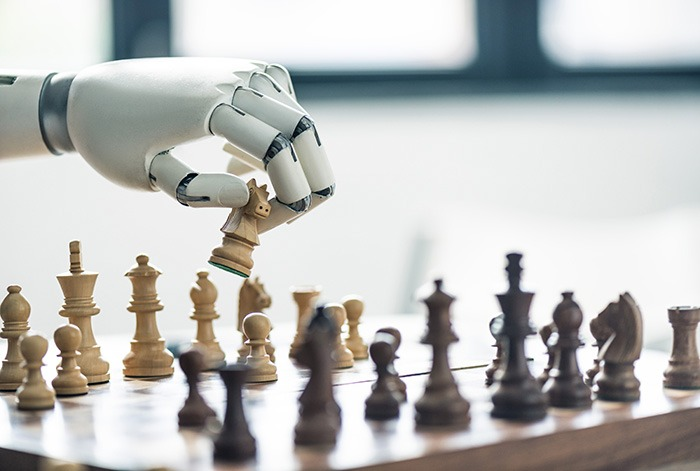
\includegraphics[width=0.38\textwidth]{slike/robotsah.jpg}
\end{wrapfigure}

Вештачка интелигенција (\textbf{AI}) представља једну од најважнијих области савремене информатике. 
Њена примена у шаху показује како рачунари могу доносити сложене одлуке.

\textit{Шах} је идеалан за тестирање алгоритама јер има јасна правила и огроман број могућих позиција.

\section{Историја}

\subsection{Рани развој}

Први програми за шах развијени су средином 20. века.

\subsection{Deep Blue}

Године 1997. рачунар је победио светског шампиона.
Позната формула из физике:
\[
E = mc^2
\]

\section{Како ради AI}

\subsection{Алгоритми}

\begin{itemize}
    \item Минимакс алгоритам
    \item Алфа-бета одсецање
    \item Хеуристике
\end{itemize}

\subsection{Напредни приступи}

\begin{enumerate}
    \item Машинско учење
    \item Неуронске мреже
    \item Самостално учење (AlphaZero)
\end{enumerate}

\section{Математички модели}

\begin{definicija}
Шаховска позиција је формални опис распореда фигура на табли.
\end{definicija}

\begin{lema}
Ако је позиција добитна, постоји низ потеза који води до победе.
\end{lema}

\begin{teorema}
Минимакс алгоритам гарантује оптималан потез ако се претражи цело стабло игре.
\end{teorema}

\section{Поређење система}

\begin{table}[h!]
\centering
\begin{tabular}{|c|c|c|}
\hline
Систем & Година & Карактеристике \\
\hline
Deep Blue & 1997 & Победио шампиона \\
Stockfish & 2008 & Отворен код \\
AlphaZero & 2017 & Самостално учење \\
\hline
\end{tabular}
\caption{Поређење AI система}
\end{table}

\section{Форматирање текста}

Ово је \textbf{подебљан текст}.

Ово је \textit{курзив текст}.

Ово је {\color{blue}обојен текст}.

\section{Закључак}

Вештачка интелигенција у шаху показује велики напредак технологије.
Очекује се да ће будући системи бити још напреднији и применљиви у другим областима.

\end{document}